\documentclass[aspectratio=169]{beamer}
% Add slides directory to search path for Dartmouth theme
\makeatletter
\def\input@path{{../}}
\makeatother
\usetheme{Dartmouth}
\usepackage{booktabs}
\usepackage{listings}
\usepackage{tikz}
\usetikzlibrary{arrows.meta,positioning,shapes,decorations.pathreplacing}
\usepackage{hyperref}
\usepackage{xcolor}
\usepackage{graphicx}
\usepackage{fontspec}
\usepackage{tcolorbox}
\usepackage{amsmath}
\usepackage{amssymb}

% Color scheme
\definecolor{darkblue}{RGB}{0,82,155}
\definecolor{lightblue}{RGB}{100,181,246}
\definecolor{darkgreen}{RGB}{46,125,50}
\definecolor{orange}{RGB}{255,152,0}
\definecolor{purple}{RGB}{142,36,170}
\definecolor{thinkbox}{RGB}{255,245,220}
\definecolor{discussbox}{RGB}{230,240,255}

\setbeamercolor{frametitle}{bg=darkblue}
\setbeamercolor{progress bar}{fg=lightblue,bg=lightblue!30}

% Code listing settings
\lstset{
    basicstyle=\ttfamily\scriptsize,
    breaklines=true,
    frame=single,
    backgroundcolor=\color{gray!10},
    keywordstyle=\color{darkblue}\bfseries,
    commentstyle=\color{darkgreen}\itshape,
    stringstyle=\color{orange},
    showstringspaces=false,
    language=Python,
    numbers=left,
    numberstyle=\tiny\color{gray}
}

% Custom boxes
\newtcolorbox{thinkaboutit}{
    colback=thinkbox,
    colframe=orange,
    title=💭 Think about it!,
    fonttitle=\bfseries
}

\newtcolorbox{discussion}{
    colback=discussbox,
    colframe=blue,
    title=💬 Discussion,
    fonttitle=\bfseries
}

\title{Lecture 20: Implementing GPT from Scratch}
\subtitle{Building a Language Model in PyTorch 💻}
\author{Models of Language and Conversation}
\institute{Dr. Jeremy R. Manning}
\date{Week 7}

\begin{document}

% Title slide
\begin{frame}
    \titlepage
\end{frame}

% Table of contents
\begin{frame}{Today's Journey 🗺️}
    \tableofcontents
\end{frame}

\section{Overview and Setup}

\begin{frame}[shrink=10]{What We'll Build Today 🏗️}
\small
    \begin{alertblock}{Goal}
        Implement a simplified GPT model from scratch in PyTorch!
    \end{alertblock}

    \vspace{0.3cm}

    \textbf{Components we'll cover:}
    \begin{enumerate}\setlength{\itemsep}{0pt}
        \item 🔤 Tokenization (Byte-Pair Encoding)
        \item 📦 Embeddings (token + position)
        \item 👁️ Masked Multi-Head Attention
        \item 🧠 Transformer Decoder Block
        \item 🎯 Language Model Head
        \item 🎓 Training Loop
        \item 🎲 Text Generation
    \end{enumerate}

    \vspace{0.3cm}

    \begin{thinkaboutit}
        We'll build a "nano-GPT"—small enough to train on a laptop, but with the same architecture as the real thing!
    \end{thinkaboutit}
\end{frame}

\begin{frame}[fragile]{Required Libraries 📚}
\begin{lstlisting}[language=Python]
import torch
import torch.nn as nn
import torch.nn.functional as F
from torch.utils.data import Dataset, DataLoader
import numpy as np
import tiktoken  # OpenAI's BPE tokenizer

# Check for GPU
device = 'cuda' if torch.cuda.is_available() else 'cpu'
print(f"Using device: {device}")

# Hyperparameters
config = {
    'vocab_size': 50257,      # GPT-2 vocabulary size
    'd_model': 384,            # Embedding dimension
    'n_layers': 6,             # Number of transformer blocks
    'n_heads': 6,              # Number of attention heads
    'max_seq_len': 256,        # Maximum sequence length
    'dropout': 0.1,
    'batch_size': 32,
    'learning_rate': 3e-4,
    'num_epochs': 10
}
\end{lstlisting}

\vspace{0.3cm}
\small
\textit{Install: pip install torch tiktoken}
\end{frame}

\section{Tokenization}

\begin{frame}[shrink=10]{What is Tokenization? 🔤}
\small
    \begin{block}{Tokenization}
        Converting text into a sequence of integer IDs that the model can process.
    \end{block}

    \vspace{0.3cm}

    \textbf{Common strategies:}
    \begin{enumerate}\setlength{\itemsep}{0pt}
        \item \textbf{Word-level}: Split on spaces
        \begin{itemize}\setlength{\itemsep}{0pt}
            \item ❌ Huge vocabulary, can't handle unknown words
        \end{itemize}

        \item \textbf{Character-level}: Individual characters
        \begin{itemize}\setlength{\itemsep}{0pt}
            \item ❌ Very long sequences, loses word structure
        \end{itemize}

        \item \textbf{Subword-level (BPE)}: Best of both worlds! ✅
        \begin{itemize}\setlength{\itemsep}{0pt}
            \item Frequent words: one token
            \item Rare words: multiple subword tokens
            \item Can handle any word via character fallback
        \end{itemize}
    \end{enumerate}
\end{frame}

\begin{frame}[shrink=10]{Byte-Pair Encoding (BPE) 🧩}
    \textbf{How BPE works:}

    \vspace{0.3cm}

    \begin{enumerate}\setlength{\itemsep}{0pt}
        \item Start with characters as base vocabulary
        \item Find most frequent pair of adjacent tokens
        \item Merge this pair into a new token
        \item Repeat until desired vocabulary size
    \end{enumerate}

    \vspace{0.3cm}

    \begin{block}{Example}
        \small
        \textbf{Text:} "low low low lower lower newest newest"

        \vspace{0.3cm}

        \textbf{Iterations:}
        \begin{enumerate}\setlength{\itemsep}{0pt}
            \item Merge "l" + "o" → "lo"
            \item Merge "lo" + "w" → "low"
            \item Merge "low" + "e" + "r" → "lower"
            \item Merge "n" + "e" + "w" + "e" + "s" + "t" → "newest"
        \end{enumerate}

        \vspace{0.3cm}

        \textbf{Vocabulary:} [l, o, w, e, r, n, s, t, lo, low, lower, newest, ...]
    \end{block}
\end{frame}

\begin{frame}[fragile]{BPE Tokenization in Code 💻}
\begin{lstlisting}[language=Python]
import tiktoken

# Load GPT-2 tokenizer (uses BPE)
tokenizer = tiktoken.get_encoding("gpt2")

# Example text
text = "Hello, how are you doing today?"

# Encode: text -> token IDs
tokens = tokenizer.encode(text)
print("Tokens:", tokens)
# Output: [15496, 11, 703, 389, 345, 1804, 1909, 30]

# Decode: token IDs -> text
decoded = tokenizer.decode(tokens)
print("Decoded:", decoded)
# Output: "Hello, how are you doing today?"

# See individual token strings
for token_id in tokens:
    token_str = tokenizer.decode([token_id])
    print(f"{token_id}: '{token_str}'")

# Vocabulary size
print(f"Vocab size: {tokenizer.n_vocab}")  # 50257
\end{lstlisting}
\end{frame}

\begin{frame}[fragile]{Creating a Text Dataset 📚}
\begin{lstlisting}[language=Python]
class TextDataset(Dataset):
    def __init__(self, text_file, tokenizer, max_seq_len):
        # Load text
        with open(text_file, 'r', encoding='utf-8') as f:
            text = f.read()

        # Tokenize entire text
        self.tokens = tokenizer.encode(text)
        self.max_seq_len = max_seq_len

    def __len__(self):
        # Number of sequences we can extract
        return len(self.tokens) - self.max_seq_len

    def __getitem__(self, idx):
        # Get sequence of length max_seq_len + 1
        # (we need +1 for the target)
        chunk = self.tokens[idx:idx + self.max_seq_len + 1]

        # Input: all but last token
        x = torch.tensor(chunk[:-1], dtype=torch.long)
        # Target: all but first token
        y = torch.tensor(chunk[1:], dtype=torch.long)

        return x, y

# Usage
dataset = TextDataset('shakespeare.txt', tokenizer, config['max_seq_len'])
dataloader = DataLoader(dataset, batch_size=config['batch_size'], shuffle=True)
\end{lstlisting}
\end{frame}

\section{Model Components}

\begin{frame}[fragile]{Token and Position Embeddings 📦}
\begin{lstlisting}[language=Python]
class Embeddings(nn.Module):
    def __init__(self, vocab_size, d_model, max_seq_len, dropout):
        super().__init__()
        # Token embeddings: map token IDs to vectors
        self.token_embed = nn.Embedding(vocab_size, d_model)

        # Position embeddings: encode position information
        self.pos_embed = nn.Embedding(max_seq_len, d_model)

        self.dropout = nn.Dropout(dropout)
        self.d_model = d_model

    def forward(self, x):
        # x shape: (batch_size, seq_len)
        seq_len = x.size(1)

        # Token embeddings
        tok_emb = self.token_embed(x)  # (batch, seq_len, d_model)

        # Position embeddings
        positions = torch.arange(0, seq_len, device=x.device)
        pos_emb = self.pos_embed(positions)  # (seq_len, d_model)

        # Combine (broadcasting handles batch dimension)
        embeddings = tok_emb + pos_emb

        return self.dropout(embeddings)
\end{lstlisting}
\end{frame}

\begin{frame}[fragile]{Masked Multi-Head Attention 👁️}
\begin{lstlisting}[language=Python]
class MultiHeadAttention(nn.Module):
    def __init__(self, d_model, n_heads, dropout):
        super().__init__()
        assert d_model % n_heads == 0

        self.d_model = d_model
        self.n_heads = n_heads
        self.head_dim = d_model // n_heads

        # Linear layers for Q, K, V
        self.q_linear = nn.Linear(d_model, d_model)
        self.k_linear = nn.Linear(d_model, d_model)
        self.v_linear = nn.Linear(d_model, d_model)

        # Output projection
        self.out_linear = nn.Linear(d_model, d_model)
        self.dropout = nn.Dropout(dropout)

    def forward(self, x, mask=None):
        batch_size, seq_len, d_model = x.shape

        # Linear projections and split into heads
        Q = self.q_linear(x).view(batch_size, seq_len, self.n_heads, self.head_dim)
        K = self.k_linear(x).view(batch_size, seq_len, self.n_heads, self.head_dim)
        V = self.v_linear(x).view(batch_size, seq_len, self.n_heads, self.head_dim)

        # Transpose for attention: (batch, n_heads, seq_len, head_dim)
        Q = Q.transpose(1, 2)
        K = K.transpose(1, 2)
        V = V.transpose(1, 2)
\end{lstlisting}
\end{frame}

\begin{frame}[fragile]{Attention Computation (cont.) 🧮}
\begin{lstlisting}[language=Python]
        # Scaled dot-product attention
        # Scores: (batch, n_heads, seq_len, seq_len)
        scores = torch.matmul(Q, K.transpose(-2, -1)) / np.sqrt(self.head_dim)

        # Apply causal mask (prevent attending to future tokens)
        if mask is not None:
            scores = scores.masked_fill(mask == 0, float('-inf'))

        # Softmax to get attention weights
        attn_weights = F.softmax(scores, dim=-1)
        attn_weights = self.dropout(attn_weights)

        # Apply attention to values
        # Output: (batch, n_heads, seq_len, head_dim)
        attn_output = torch.matmul(attn_weights, V)

        # Concatenate heads
        attn_output = attn_output.transpose(1, 2).contiguous()
        attn_output = attn_output.view(batch_size, seq_len, d_model)

        # Final linear projection
        output = self.out_linear(attn_output)

        return output
\end{lstlisting}
\end{frame}

\begin{frame}[fragile]{Creating the Causal Mask 🎭}
\begin{lstlisting}[language=Python]
def create_causal_mask(seq_len, device):
    """
    Create a causal (lower-triangular) mask for autoregressive generation.

    Returns:
        mask: (seq_len, seq_len) with 1s on and below diagonal, 0s above
    """
    mask = torch.tril(torch.ones(seq_len, seq_len, device=device))
    return mask  # Shape: (seq_len, seq_len)

# Example: 5x5 causal mask
mask = create_causal_mask(5, 'cpu')
print(mask)
# tensor([[1., 0., 0., 0., 0.],
#         [1., 1., 0., 0., 0.],
#         [1., 1., 1., 0., 0.],
#         [1., 1., 1., 1., 0.],
#         [1., 1., 1., 1., 1.]])
\end{lstlisting}

\vspace{0.3cm}

\textbf{Key insight:} Each position can only attend to itself and previous positions!
\end{frame}

\begin{frame}[fragile]{Feed-Forward Network 🔄}
\begin{lstlisting}[language=Python]
class FeedForward(nn.Module):
    def __init__(self, d_model, dropout):
        super().__init__()
        # GPT uses 4 * d_model as the hidden dimension
        self.net = nn.Sequential(
            nn.Linear(d_model, 4 * d_model),
            nn.GELU(),  # GPT uses GELU activation
            nn.Linear(4 * d_model, d_model),
            nn.Dropout(dropout)
        )

    def forward(self, x):
        return self.net(x)
\end{lstlisting}

\vspace{0.3cm}

\textbf{Why GELU (Gaussian Error Linear Unit)?}
\begin{itemize}\setlength{\itemsep}{0pt}
    \item Smooth, non-monotonic activation
    \item Used in BERT and GPT
    \item Slight improvement over ReLU for language models
\end{itemize}

\vspace{0.3cm}

$$\text{GELU}(x) = x \cdot \Phi(x) = x \cdot \frac{1}{2}\left[1 + \text{erf}\left(\frac{x}{\sqrt{2}}\right)\right]$$
\end{frame}

\begin{frame}[fragile]{Transformer Decoder Block 🧱}
\begin{lstlisting}[language=Python]
class TransformerBlock(nn.Module):
    def __init__(self, d_model, n_heads, dropout):
        super().__init__()
        self.attention = MultiHeadAttention(d_model, n_heads, dropout)
        self.feed_forward = FeedForward(d_model, dropout)

        # Layer normalization (applied before sub-layers in GPT)
        self.ln1 = nn.LayerNorm(d_model)
        self.ln2 = nn.LayerNorm(d_model)

    def forward(self, x, mask):
        # Pre-norm architecture (used in GPT)
        # Attention with residual connection
        x = x + self.attention(self.ln1(x), mask)

        # Feed-forward with residual connection
        x = x + self.feed_forward(self.ln2(x))

        return x
\end{lstlisting}

\vspace{0.3cm}

\textbf{Note:} GPT uses \textit{pre-norm} (LayerNorm before sub-layers), while original Transformer used \textit{post-norm}.
\end{frame}

\begin{frame}[fragile]{Complete GPT Model 🤖}
\begin{lstlisting}[language=Python]
class GPT(nn.Module):
    def __init__(self, vocab_size, d_model, n_layers, n_heads, max_seq_len, dropout):
        super().__init__()
        self.max_seq_len = max_seq_len

        # Embeddings
        self.embeddings = Embeddings(vocab_size, d_model, max_seq_len, dropout)

        # Transformer blocks
        self.blocks = nn.ModuleList([
            TransformerBlock(d_model, n_heads, dropout)
            for _ in range(n_layers)
        ])

        # Final layer norm
        self.ln_f = nn.LayerNorm(d_model)

        # Language model head (projects to vocabulary)
        self.lm_head = nn.Linear(d_model, vocab_size, bias=False)

        # Initialize weights
        self.apply(self._init_weights)

    def _init_weights(self, module):
        if isinstance(module, nn.Linear):
            torch.nn.init.normal_(module.weight, mean=0.0, std=0.02)
            if module.bias is not None:
                torch.nn.init.zeros_(module.bias)
        elif isinstance(module, nn.Embedding):
            torch.nn.init.normal_(module.weight, mean=0.0, std=0.02)
\end{lstlisting}
\end{frame}

\begin{frame}[fragile]{GPT Forward Pass 🔜}
\begin{lstlisting}[language=Python]
    def forward(self, x, targets=None):
        # x shape: (batch_size, seq_len)
        seq_len = x.size(1)

        # Create causal mask
        mask = create_causal_mask(seq_len, x.device)

        # Embeddings
        x = self.embeddings(x)  # (batch, seq_len, d_model)

        # Apply transformer blocks
        for block in self.blocks:
            x = block(x, mask)

        # Final layer norm
        x = self.ln_f(x)

        # Project to vocabulary
        logits = self.lm_head(x)  # (batch, seq_len, vocab_size)

        # Compute loss if targets provided
        loss = None
        if targets is not None:
            # Flatten for cross-entropy
            loss = F.cross_entropy(
                logits.view(-1, logits.size(-1)),
                targets.view(-1)
            )

        return logits, loss
\end{lstlisting}
\end{frame}

\section{Training}

\begin{frame}[fragile]{Training Loop 🎓}
\begin{lstlisting}[language=Python]
# Initialize model
model = GPT(
    vocab_size=config['vocab_size'],
    d_model=config['d_model'],
    n_layers=config['n_layers'],
    n_heads=config['n_heads'],
    max_seq_len=config['max_seq_len'],
    dropout=config['dropout']
).to(device)

# Optimizer (AdamW is used for GPT)
optimizer = torch.optim.AdamW(
    model.parameters(),
    lr=config['learning_rate'],
    betas=(0.9, 0.95),
    weight_decay=0.1
)

# Training loop
model.train()
for epoch in range(config['num_epochs']):
    total_loss = 0
    for batch_idx, (x, y) in enumerate(dataloader):
        x, y = x.to(device), y.to(device)

        # Forward pass
        logits, loss = model(x, targets=y)

        # Backward pass
        optimizer.zero_grad()
        loss.backward()
        torch.nn.utils.clip_grad_norm_(model.parameters(), 1.0)
        optimizer.step()

        total_loss += loss.item()

    avg_loss = total_loss / len(dataloader)
    print(f"Epoch {epoch+1}/{config['num_epochs']}, Loss: {avg_loss:.4f}")
\end{lstlisting}
\end{frame}

\begin{frame}[shrink=10]{Training Tips 💡}
    \textbf{Best practices for training GPT:}

    \vspace{0.3cm}

    \begin{enumerate}\setlength{\itemsep}{0pt}
        \item \textbf{Gradient clipping}
        \begin{itemize}\setlength{\itemsep}{0pt}
            \item Prevents exploding gradients
            \item Clip to max norm of 1.0
        \end{itemize}

        \item \textbf{Learning rate schedule}
        \begin{itemize}\setlength{\itemsep}{0pt}
            \item Warmup for first few thousand steps
            \item Cosine decay afterwards
        \end{itemize}

        \item \textbf{AdamW optimizer}
        \begin{itemize}\setlength{\itemsep}{0pt}
            \item Adam with decoupled weight decay
            \item Better than standard Adam for transformers
        \end{itemize}

        \item \textbf{Batch size}
        \begin{itemize}\setlength{\itemsep}{0pt}
            \item Larger is better (up to memory limits)
            \item Use gradient accumulation if needed
        \end{itemize}

        \item \textbf{Mixed precision training}
        \begin{itemize}\setlength{\itemsep}{0pt}
            \item Use float16 for speed
            \item 2-3x faster on modern GPUs
        \end{itemize}
    \end{enumerate}
\end{frame}

\section{Text Generation}

\begin{frame}[fragile]{Greedy Decoding 🎯}
\begin{lstlisting}[language=Python]
@torch.no_grad()
def generate_greedy(model, tokenizer, prompt, max_new_tokens=50):
    model.eval()

    # Encode prompt
    tokens = tokenizer.encode(prompt)
    x = torch.tensor([tokens], dtype=torch.long, device=device)

    for _ in range(max_new_tokens):
        # Get predictions (crop to max_seq_len if needed)
        x_crop = x[:, -model.max_seq_len:]
        logits, _ = model(x_crop)

        # Focus on last token's predictions
        logits = logits[:, -1, :]  # (batch, vocab_size)

        # Get token with highest probability
        next_token = torch.argmax(logits, dim=-1, keepdim=True)

        # Append to sequence
        x = torch.cat([x, next_token], dim=1)

        # Stop if we generate end-of-sequence token
        if next_token.item() == tokenizer.eot_token:
            break

    # Decode and return
    generated_text = tokenizer.decode(x[0].tolist())
    return generated_text

# Example usage
prompt = "Once upon a time"
generated = generate_greedy(model, tokenizer, prompt, max_new_tokens=100)
print(generated)
\end{lstlisting}
\end{frame}

\begin{frame}[shrink=10]{Sampling Strategies 🎲}
    \textbf{Different ways to sample next token:}

    \vspace{0.3cm}

    \begin{enumerate}\setlength{\itemsep}{0pt}
        \item \textbf{Greedy Decoding}
        \begin{itemize}\setlength{\itemsep}{0pt}
            \item Always pick most likely token
            \item ✅ Deterministic, fast
            \item ❌ Repetitive, boring
        \end{itemize}

        \item \textbf{Temperature Sampling}
        \begin{itemize}\setlength{\itemsep}{0pt}
            \item Scale logits by temperature $T$
            \item $T < 1$: More conservative (peaked distribution)
            \item $T > 1$: More random (flat distribution)
        \end{itemize}

        \item \textbf{Top-k Sampling}
        \begin{itemize}\setlength{\itemsep}{0pt}
            \item Sample from top $k$ most likely tokens
            \item Typical: $k = 40$
        \end{itemize}

        \item \textbf{Nucleus (Top-p) Sampling}
        \begin{itemize}\setlength{\itemsep}{0pt}
            \item Sample from smallest set with cumulative probability $\geq p$
            \item Typical: $p = 0.9$ or $p = 0.95$
            \item ✅ Best for creative generation
        \end{itemize}
    \end{enumerate}
\end{frame}

\begin{frame}[fragile]{Top-k and Nucleus Sampling 🎰}
\begin{lstlisting}[language=Python]
def sample_next_token(logits, temperature=1.0, top_k=None, top_p=None):
    """
    Sample next token from logits with various strategies.

    Args:
        logits: (vocab_size,) unnormalized log probabilities
        temperature: Temperature for sampling
        top_k: If set, only sample from top k tokens
        top_p: If set, only sample from nucleus (top-p)
    """
    # Apply temperature
    logits = logits / temperature

    # Top-k filtering
    if top_k is not None:
        top_k = min(top_k, logits.size(-1))
        indices_to_remove = logits < torch.topk(logits, top_k)[0][..., -1, None]
        logits[indices_to_remove] = float('-inf')

    # Nucleus (top-p) filtering
    if top_p is not None:
        sorted_logits, sorted_indices = torch.sort(logits, descending=True)
        cumulative_probs = torch.cumsum(F.softmax(sorted_logits, dim=-1), dim=-1)

        # Remove tokens with cumulative probability above threshold
        sorted_indices_to_remove = cumulative_probs > top_p
        sorted_indices_to_remove[..., 1:] = sorted_indices_to_remove[..., :-1].clone()
        sorted_indices_to_remove[..., 0] = 0

        indices_to_remove = sorted_indices[sorted_indices_to_remove]
        logits[indices_to_remove] = float('-inf')

    # Sample from distribution
    probs = F.softmax(logits, dim=-1)
    next_token = torch.multinomial(probs, num_samples=1)

    return next_token
\end{lstlisting}
\end{frame}

\begin{frame}[fragile]{Complete Generation Function 🎨}
\begin{lstlisting}[language=Python]
@torch.no_grad()
def generate(model, tokenizer, prompt, max_new_tokens=100,
             temperature=1.0, top_k=40, top_p=0.9):
    model.eval()

    tokens = tokenizer.encode(prompt)
    x = torch.tensor([tokens], dtype=torch.long, device=device)

    for _ in range(max_new_tokens):
        x_crop = x[:, -model.max_seq_len:]
        logits, _ = model(x_crop)
        logits = logits[:, -1, :]  # Last token

        # Sample next token
        next_token = sample_next_token(
            logits[0],
            temperature=temperature,
            top_k=top_k,
            top_p=top_p
        )

        x = torch.cat([x, next_token.unsqueeze(0)], dim=1)

        if next_token.item() == tokenizer.eot_token:
            break

    return tokenizer.decode(x[0].tolist())

# Creative generation
text = generate(model, tokenizer, "The AI revolution",
                temperature=0.8, top_p=0.9)
print(text)
\end{lstlisting}
\end{frame}

\section{Practical Considerations}

\begin{frame}[shrink=5]{Model Size vs. Performance 📊}
    \begin{center}
        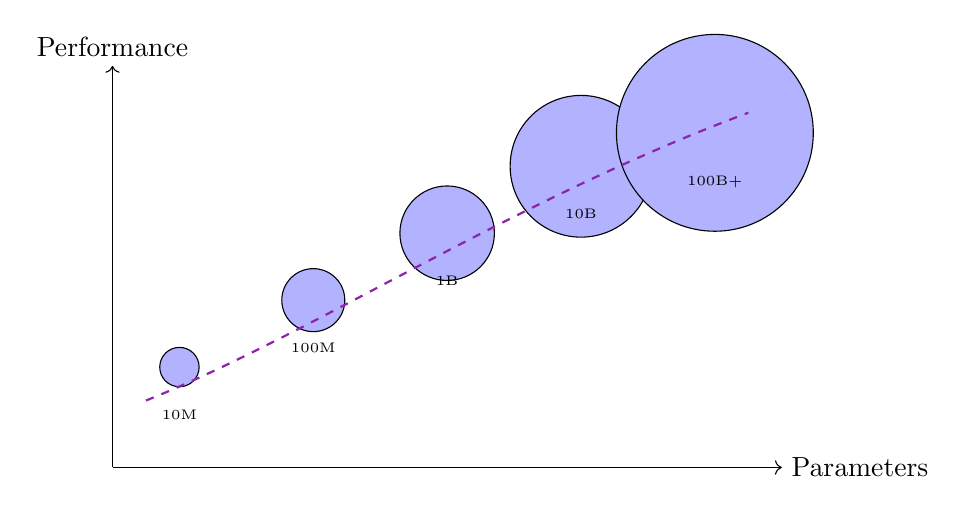
\begin{tikzpicture}[scale=0.85]
            % Axes
            \draw[->] (0,0) -- (10,0) node[right] {Parameters};
            \draw[->] (0,0) -- (0,6) node[above] {Performance};

            % Models
            \node[circle, draw, fill=blue!30, minimum size=0.5cm] at (1,1.5) {};
            \node[below] at (1,1) {\tiny 10M};

            \node[circle, draw, fill=blue!30, minimum size=0.8cm] at (3,2.5) {};
            \node[below] at (3,2) {\tiny 100M};

            \node[circle, draw, fill=blue!30, minimum size=1.2cm] at (5,3.5) {};
            \node[below] at (5,3) {\tiny 1B};

            \node[circle, draw, fill=blue!30, minimum size=1.8cm] at (7,4.5) {};
            \node[below] at (7,4) {\tiny 10B};

            \node[circle, draw, fill=blue!30, minimum size=2.5cm] at (9,5) {};
            \node[below] at (9,4.5) {\tiny 100B+};

            % Curve
            \draw[thick, purple, dashed] (0.5,1) .. controls (3,2) and (6,4) .. (9.5,5.3);
        \end{tikzpicture}
    \end{center}

    \vspace{0.3cm}

    \textbf{Practical model sizes for different use cases:}
    \begin{itemize}\setlength{\itemsep}{0pt}
        \item \textbf{10M-100M}: Learning/experimentation, simple tasks
        \item \textbf{100M-1B}: Specialized domains, resource-constrained
        \item \textbf{1B-10B}: General-purpose, good quality
        \item \textbf{10B-100B+}: State-of-the-art performance
    \end{itemize}
\end{frame}

\begin{frame}{Computational Requirements 💻}
\small
    \textbf{Training a 125M parameter GPT:}

    \vspace{0.3cm}

    \begin{table}
        \begin{tabular}{ll}
            \toprule
            \textbf{Resource} & \textbf{Amount} \\
            \midrule
            GPU Memory & $\sim$8-12 GB \\
            Training Time & 1-2 days (single GPU) \\
            Training Data & $\sim$10-100 GB text \\
            Total Compute & $\sim$100 GPU-hours \\
            \bottomrule
        \end{tabular}
    \end{table}

    \vspace{0.3cm}

    \textbf{Scaling up to GPT-3 (175B):}
    \begin{itemize}\setlength{\itemsep}{0pt}
        \item 1000x more parameters
        \item ~10,000x more compute needed
        \item Requires distributed training across many GPUs
        \item Estimated \$4.6M in compute costs
    \end{itemize}

    \vspace{0.3cm}

    \begin{thinkaboutit}
        This is why pre-trained models are so valuable—you don't have to train from scratch!
    \end{thinkaboutit}
\end{frame}

\begin{frame}[shrink=10]{Common Issues and Debugging 🔧}
    \textbf{Problems you might encounter:}

    \vspace{0.3cm}

    \begin{enumerate}\setlength{\itemsep}{0pt}
        \item \textbf{Loss not decreasing}
        \begin{itemize}\setlength{\itemsep}{0pt}
            \item Check learning rate (try 1e-4 to 3e-4)
            \item Verify data pipeline
            \item Check for NaN/Inf values
        \end{itemize}

        \item \textbf{Out of memory}
        \begin{itemize}\setlength{\itemsep}{0pt}
            \item Reduce batch size
            \item Reduce sequence length
            \item Use gradient accumulation
            \item Enable mixed precision
        \end{itemize}

        \item \textbf{Poor generation quality}
        \begin{itemize}\setlength{\itemsep}{0pt}
            \item Train longer
            \item Use larger model
            \item Improve data quality
            \item Tune sampling parameters
        \end{itemize}

        \item \textbf{Repetitive text}
        \begin{itemize}\setlength{\itemsep}{0pt}
            \item Increase temperature
            \item Use nucleus sampling
            \item Add repetition penalty
        \end{itemize}
    \end{enumerate}
\end{frame}

\begin{frame}[shrink=10]{Extensions and Improvements 🚀}
    \textbf{Ways to enhance your GPT implementation:}

    \vspace{0.3cm}

    \begin{enumerate}\setlength{\itemsep}{0pt}
        \item \textbf{Architectural improvements}
        \begin{itemize}\setlength{\itemsep}{0pt}
            \item Rotary Position Embeddings (RoPE)
            \item Flash Attention (faster attention)
            \item Grouped-Query Attention
        \end{itemize}

        \item \textbf{Training techniques}
        \begin{itemize}\setlength{\itemsep}{0pt}
            \item Learning rate warmup and decay
            \item Gradient accumulation
            \item Mixed precision training (FP16/BF16)
        \end{itemize}

        \item \textbf{Data improvements}
        \begin{itemize}\setlength{\itemsep}{0pt}
            \item Data deduplication
            \item Quality filtering
            \item Curriculum learning
        \end{itemize}

        \item \textbf{Inference optimizations}
        \begin{itemize}\setlength{\itemsep}{0pt}
            \item KV-cache for faster generation
            \item Model quantization (int8)
            \item Speculative decoding
        \end{itemize}
    \end{enumerate}
\end{frame}

\begin{frame}[shrink=10]{Resources for Further Learning 📚}
    \textbf{Recommended resources:}

    \vspace{0.3cm}

    \begin{itemize}\setlength{\itemsep}{0pt}
        \item \textbf{Andrej Karpathy's nanoGPT}
        \begin{itemize}\setlength{\itemsep}{0pt}
            \item Clean, minimal GPT implementation
            \item \href{https://github.com/karpathy/nanoGPT}{github.com/karpathy/nanoGPT}
        \end{itemize}

        \item \textbf{Andrej Karpathy's "Let's build GPT" video}
        \begin{itemize}\setlength{\itemsep}{0pt}
            \item Excellent step-by-step tutorial
            \item \href{https://www.youtube.com/watch?v=kCc8FmEb1nY}{YouTube}
        \end{itemize}

        \item \textbf{HuggingFace Transformers}
        \begin{itemize}\setlength{\itemsep}{0pt}
            \item Production-ready implementations
            \item \href{https://huggingface.co/transformers}{huggingface.co/transformers}
        \end{itemize}

        \item \textbf{PyTorch Documentation}
        \begin{itemize}\setlength{\itemsep}{0pt}
            \item Official tutorials and guides
            \item \href{https://pytorch.org/tutorials}{pytorch.org/tutorials}
        \end{itemize}
    \end{itemize}
\end{frame}

\begin{frame}[shrink=10]{Hands-On Exercise 💪}
    \begin{alertblock}{Your Task}
        Implement and train a small GPT model on your own text corpus!
    \end{alertblock}

    \vspace{0.3cm}

    \textbf{Steps:}
    \begin{enumerate}\setlength{\itemsep}{0pt}
        \item Choose a dataset (Shakespeare, Wikipedia, your own text)
        \item Set up the data pipeline
        \item Initialize the model (start small: 6 layers, 384 d\_model)
        \item Train for 10-20 epochs
        \item Experiment with generation
        \item Try different sampling strategies
    \end{enumerate}

    \vspace{0.3cm}

    \textbf{Starter code available:}
    \begin{itemize}\setlength{\itemsep}{0pt}
        \item Course GitHub repository
        \item Google Colab notebook
        \item Estimated time: 2-3 hours
    \end{itemize}
\end{frame}

\begin{frame}[shrink=10]{Key Takeaways 🔑}
    \begin{enumerate}\setlength{\itemsep}{0pt}
        \item \textbf{GPT is conceptually simple}
        \begin{itemize}\setlength{\itemsep}{0pt}
            \item Stack of transformer decoder blocks
            \item Predict next token
        \end{itemize}

        \vspace{0.3cm}

        \item \textbf{Key components}
        \begin{itemize}\setlength{\itemsep}{0pt}
            \item BPE tokenization
            \item Token + position embeddings
            \item Masked multi-head attention
            \item Feed-forward networks
        \end{itemize}

        \vspace{0.3cm}

        \item \textbf{Training requires care}
        \begin{itemize}\setlength{\itemsep}{0pt}
            \item Good data, proper hyperparameters
            \item Gradient clipping, learning rate schedules
        \end{itemize}

        \vspace{0.3cm}

        \item \textbf{Generation is an art}
        \begin{itemize}\setlength{\itemsep}{0pt}
            \item Balance creativity and coherence
            \item Temperature, top-k, top-p sampling
        \end{itemize}

        \vspace{0.3cm}

        \item \textbf{Implementation teaches you how LLMs work}
        \begin{itemize}\setlength{\itemsep}{0pt}
            \item Understanding through building!
        \end{itemize}
    \end{enumerate}
\end{frame}

\begin{frame}[shrink=10]{Readings 📖}
\small
    \begin{block}{Required Readings}
        \begin{enumerate}\setlength{\itemsep}{0pt}
            \item \textbf{Vaswani et al. (2017)} - "Attention is All You Need" \\
            \href{https://arxiv.org/abs/1706.03762}{[ArXiv]}

            \item \textbf{Radford et al. (2018)} - "Improving Language Understanding by Generative Pre-Training" \\
            \href{https://cdn.openai.com/research-covers/language-unsupervised/language_understanding_paper.pdf}{[PDF]}
        \end{enumerate}
    \end{block}

    \vspace{0.3cm}

    \begin{block}{Code Resources}
        \begin{itemize}\setlength{\itemsep}{0pt}
            \item \textbf{nanoGPT} by Andrej Karpathy \\
            \href{https://github.com/karpathy/nanoGPT}{github.com/karpathy/nanoGPT}

            \item \textbf{The Annotated Transformer} \\
            \href{https://nlp.seas.harvard.edu/2018/04/03/attention.html}{Harvard NLP}

            \item \textbf{PyTorch Transformer Tutorial} \\
            \href{https://pytorch.org/tutorials/beginner/transformer_tutorial.html}{pytorch.org}
        \end{itemize}
    \end{block}
\end{frame}

\begin{frame}[shrink=10]{Next Week 🔮}
    \textbf{Week 8: No Classes - Instructor Away}

    \vspace{0.5cm}

    \textbf{Use this week to:}
    \begin{itemize}\setlength{\itemsep}{0pt}
        \item Complete the GPT implementation exercise
        \item Catch up on readings
        \item Work on assignments
        \item Experiment with different architectures
    \end{itemize}

    \vspace{0.5cm}

    \textbf{Week 9: RAG \& Mixture of Experts}
    \begin{itemize}\setlength{\itemsep}{0pt}
        \item Retrieval Augmented Generation
        \item Mixture of Experts architectures
        \item Ethics, Bias, and Safety in LLMs
    \end{itemize}
\end{frame}

\begin{frame}
    \begin{center}
        \Huge{Questions? 💬}

        \vspace{2cm}

        \Large{Happy Coding! 🚀}
    \end{center}
\end{frame}

\end{document}
